\documentclass{article}

\usepackage{comment}
\usepackage{graphicx}
\graphicspath{ {./images/} }




\title{HERE Technologies Research Proposal}
\author{Reinhold Ludwig, Xinming Huang, Anurag Desai}

\begin{document}
	\pagenumbering{gobble}
	\maketitle
	\newpage
	\pagenumbering{arabic}
	
	\begin{comment}	
	\begin{abstract}
		
		Mapping the surrounding environment is of utmost importance for path planning and obstacle avoidance of Autonomous Vehicles. In this paper we would like to propose an innovative system that would create a dense geometric mapping algorithm for identifying and mapping static digital markers like Traffic Signal Posts, Speed Limit Signs. Our system would also be able to classify static and dynamic obstacles, and remove dynamic obstacles from the map.
		
	\end{abstract}
	\end{comment}
	
	\section{Introduction}
	\paragraph{}
	Autonomous vehicles have the potential to revolutionize the transportation industry by drastically improving safety and efficiency of transportation. In order to navigate through complex environments the vehicles rely on wide array of sensors like Light Detection And Ranging (LiDAR), Camera, Inertial Measurement Unit (IMU), Global Navigation Satellite System (GNSS). The level of autonomy in Autonomous Driving Systems is determined by its ability to perceive and navigate in complex environments. Simultaneous Localization And Mapping (SLAM) has been an active area of research in Robotics
	\cite{durrant-whyte_simultaneous_nodate}
	\cite{bailey_simultaneous_2006}.
	To accomplish this task the system needs to sense and generate an accurate map of the environment using different SLAM techniques, find its location in the map using Monte Carlo Localization
	\cite{thrun_robust_2001}
	or Kalman filter based localizations 
	and navigate to the destination. Several approaches have been proposed 
	\cite{durrant-whyte_simultaneous_nodate}
	\cite{thrun_graph_2006},
	however the most successful one
	\cite{levinson_map-based_2007}
	was developed by Stanford Artificial Intelligence Lab. 
	
	Most of the related work conducted has been focused on very specific and constrained environments, however to achieve a fully autonomous system, the challenge of mapping large-scale environments needs to be tackled. The objective of this project is to develop a system that can not only generate a three dimensional large-scale map but also add more detailed information to the map data.
	
	\begin{comment}
	Autonomous vehicles require more information that the standard 2D map provides. It needs to understand when and where to look for traffic signals, speed limits. Even to perform a simple task like taking a turn, the autonomous vehicle requires information like where the turn only lane starts which isn't provided in standard maps. Hence we need maps that have more data that simple latitude and longitudinal data.
	Perception and navigation in complex environment requires a well defined map of the environment. LiDAR is usually used to generate a map of the environment using the 3D point cloud data. Camera's do not directly provide a depth perception but can be extremely efficient in image classification and obstacle detection.
	
	\underline{\textit{How Self driving requires more data than just the data provided by GNSS}}
	\end{comment}
	
	\section{Related Work}

	Different Mapping Techniques that have been deployed for generating map data can be broadly classified into 
	LiDAR Mapping
	\cite{levinson_robust_2010},
	Visual Mapping
	\cite{chen_combining_2017}
	and Sensor Fusion based Mapping
	\cite{silva_fusion_nodate}. 
	LiDAR based mapping is usually preferred as it generates accurate point clouds data which provide a depth perception of the image. This depth information is extremely useful in navigation. Visual mapping is primarily based on camera data. Unlike LiDARs, Cameras require ambient lighting and cannot provide depth information by default. However, cameras provide better scene segmentation and understanding
	\cite{heng_project_2018}.
	We can also use multi camera system
	\cite{geiger_stereoscan:_2011}
	to gain depth perception along with different wide field of view lenses or fisheye lenses
	\cite{cui_real-time_2018}
	to gain more information.
	The sensor fusion based approach tries to combine the data from all the sensors and generates a map that has a depth perception of LiDAR as well as better scene segmentation of Camera. Other sensors commonly used are RADAR for navigation and obstacle detection, IMU and GNSS for better localization.
	The following table lists all the advantages and drawbacks of different sensors:

	\begin{figure}
		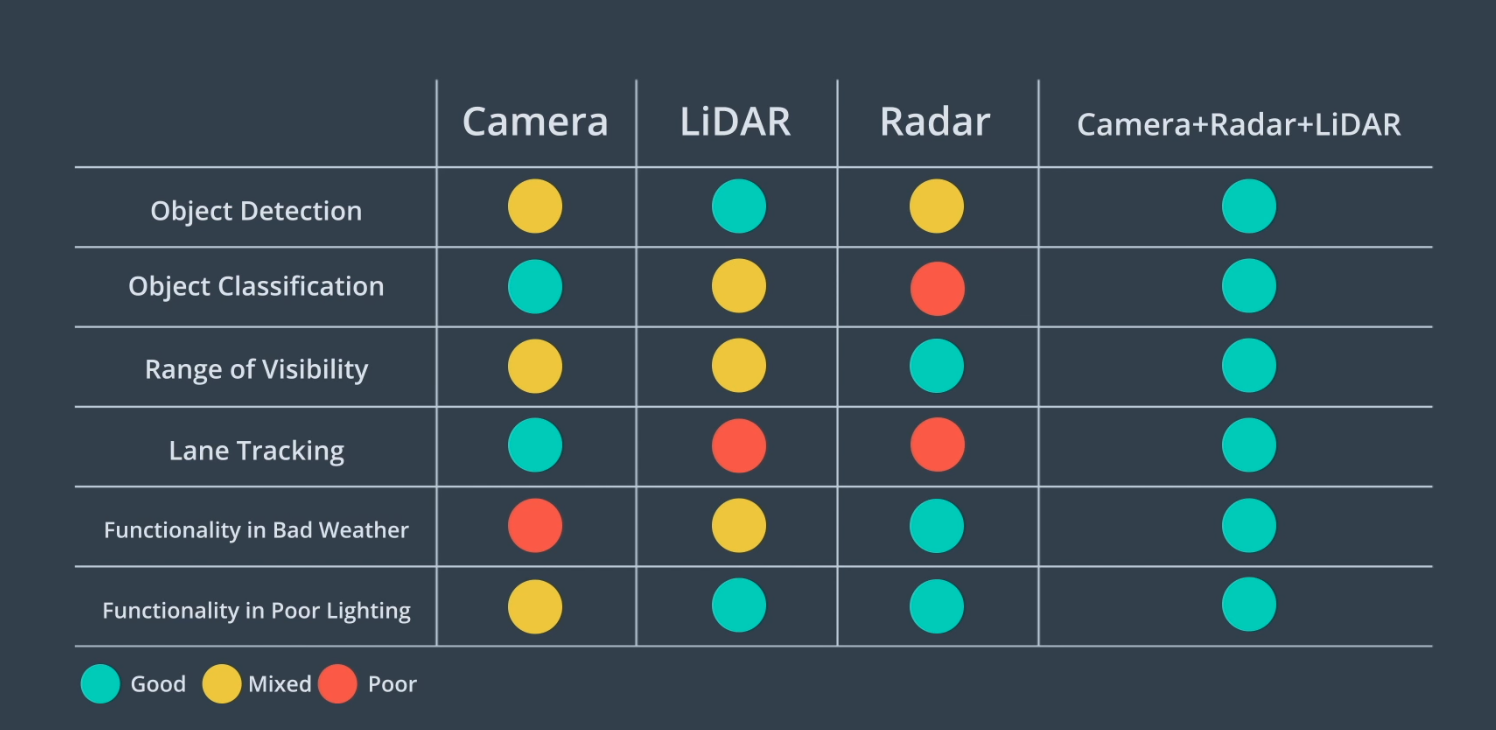
\includegraphics[width=\textwidth]{Sensor_Comparison}
		\caption{Sensor Comparison
		\cite{noauthor_self-driving_nodate}}
	\end{figure}

	
	
	
	Different ways the work load is offloaded:
	
	1. Online Method: Markov Assumption - Forget all prior data
	
	2. Offline Method: GraphSLAM, EKF-SLAM, UKF-SLAM, ISPKF-SLAM
	
	\section{Proposed Mapping Technique}
	
	We propose a 2-part system which comprises of
	
	Focus on Prior Maps usage
	
	\underline{\textit{Add references for integrating different dimensions}}
	
	On-Vehicle: for Data Recording
	
	Online Platform: for putting together the data recorded and generating a map of it
	
	ResNet Style Architecture - Use of Residual Values 
	
	\section{Conclusion}
	
	
	
\bibliography{ResearchProposal}
\bibliographystyle{IEEEtran}
\end{document}
